\section{Bandwidth}\label{sec:bandwidth}

The first group of experiments regards the bandwidth and is done using only the
topology called ``paper topology'', shown in \figref{fig:papertopo}, with only
three hosts that has to communicate. This is the topology used in the paper of
\citeauthor{ilhan-kaplan-dualascent}. For each experiment 30 results are
collected and aggregated with the average, each one using 15 seconds of TCP
traffic.

\begin{figure}[hbt]
	\centering
	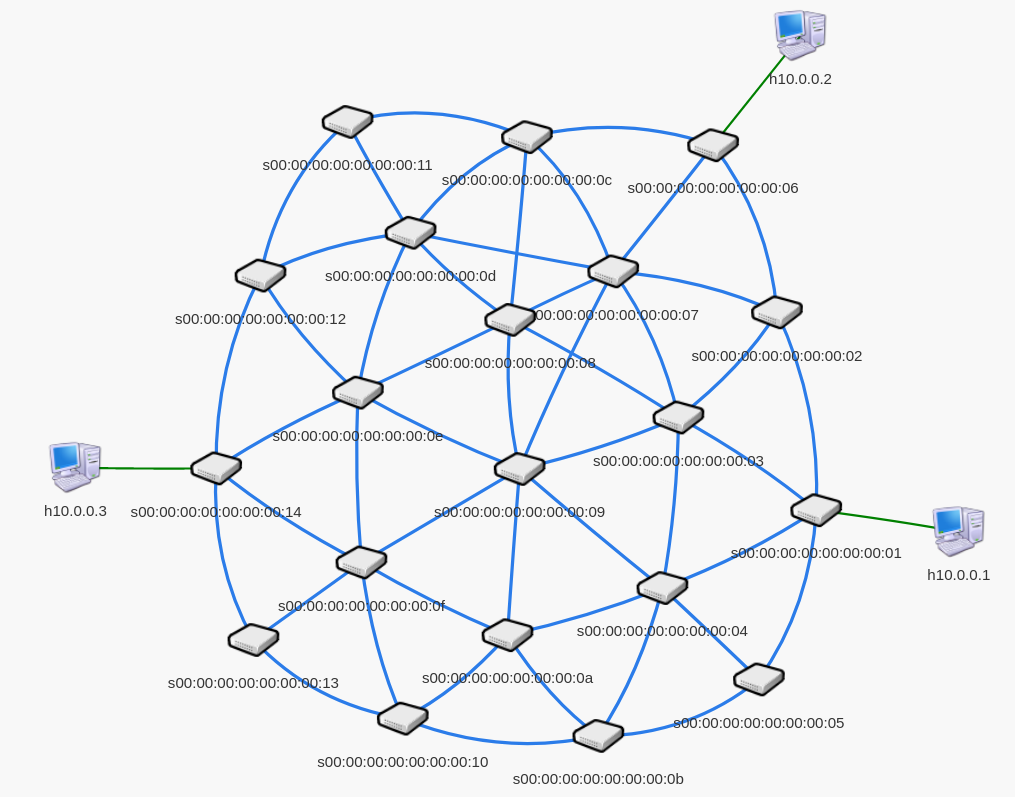
\includegraphics[width=0.8\textwidth]{img/papertopo.png}
	\caption{Paper topology}\label{fig:papertopo}
\end{figure}

\subsection{Equal link bandwidth}

For this experiment all the links hava the same bandwidth (unlimited; the only
limit is the computational limit of the CPU). In
\figref{subfig:band-eq-dijkstra} we show the various average throughputs for the
host-to-host paths in the Dijkstra's algorithm. In \figref{subfig:band-eq-dual}
we have the analogue for the dual ascent algorithm.

\begin{figure}
	\centering
	\begin{subfigure}[b]{\textwidth}
		\centering
		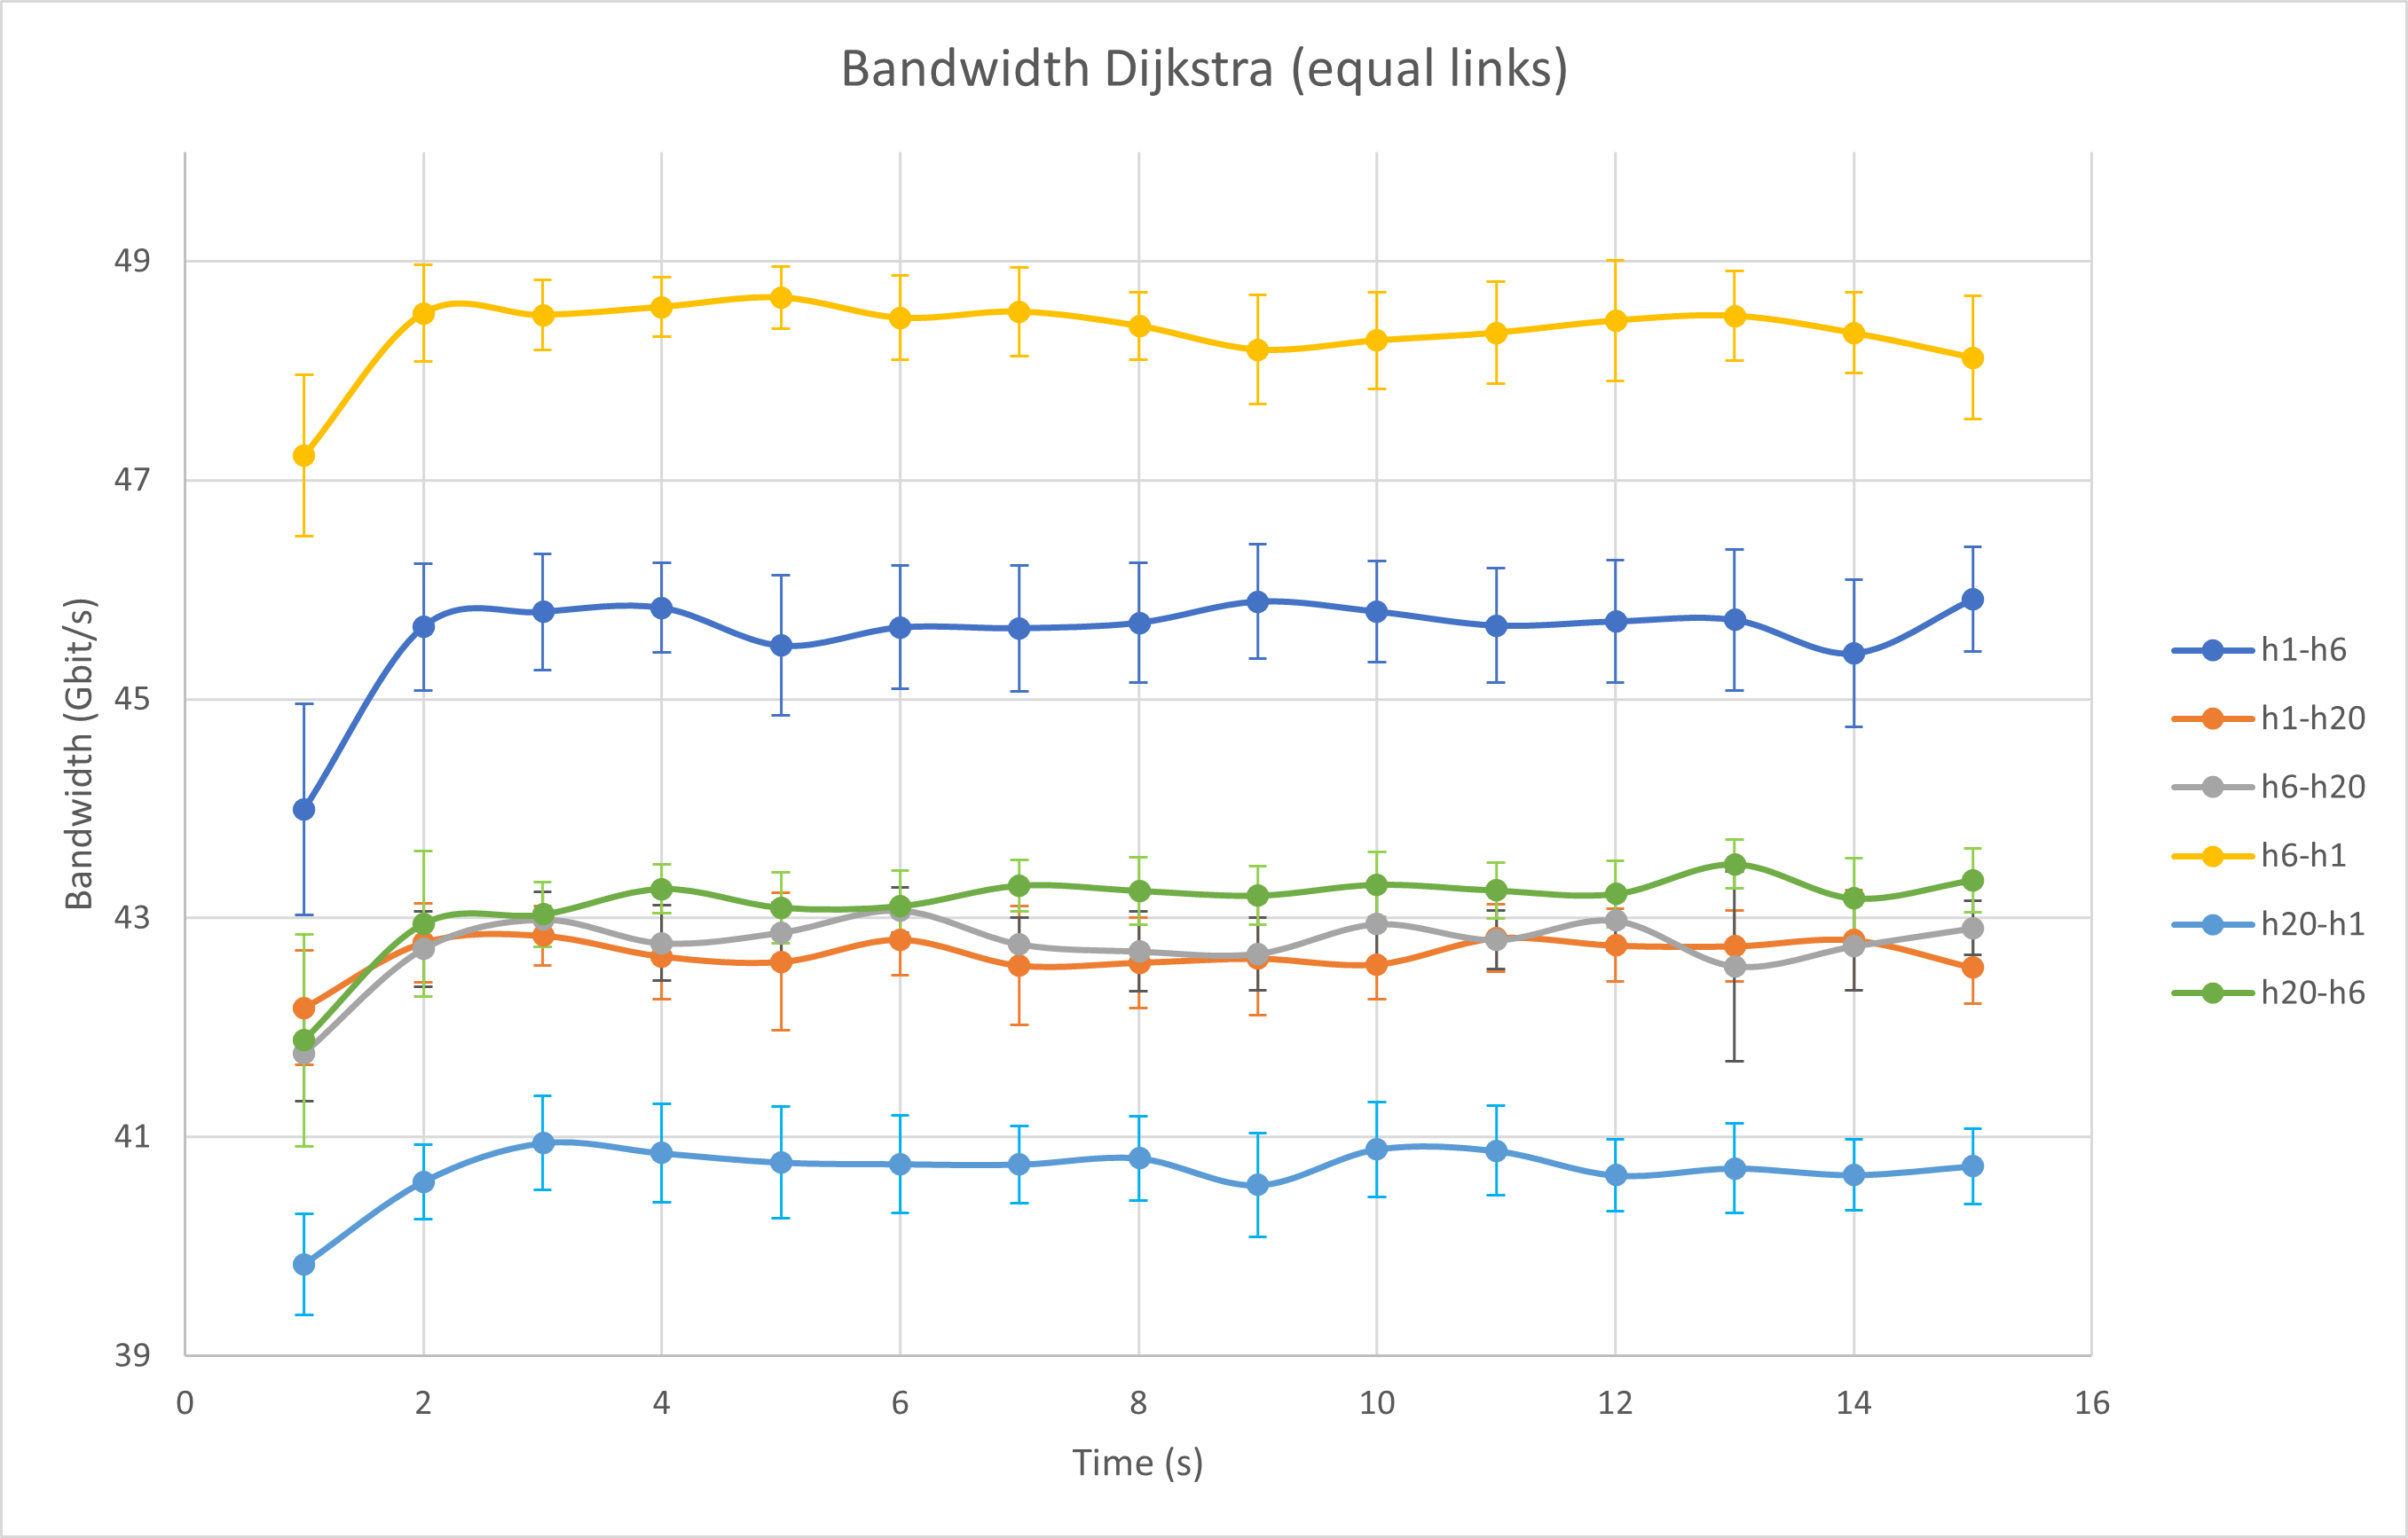
\includegraphics[width=\textwidth]{img/band-eq-dijkstra.png}
		\caption{Throughput in time for Dijkstra algorithm with equal
		link bandwidth}\label{subfig:band-eq-dijkstra}
	\end{subfigure}
	\begin{subfigure}[b]{\textwidth}
		\centering
		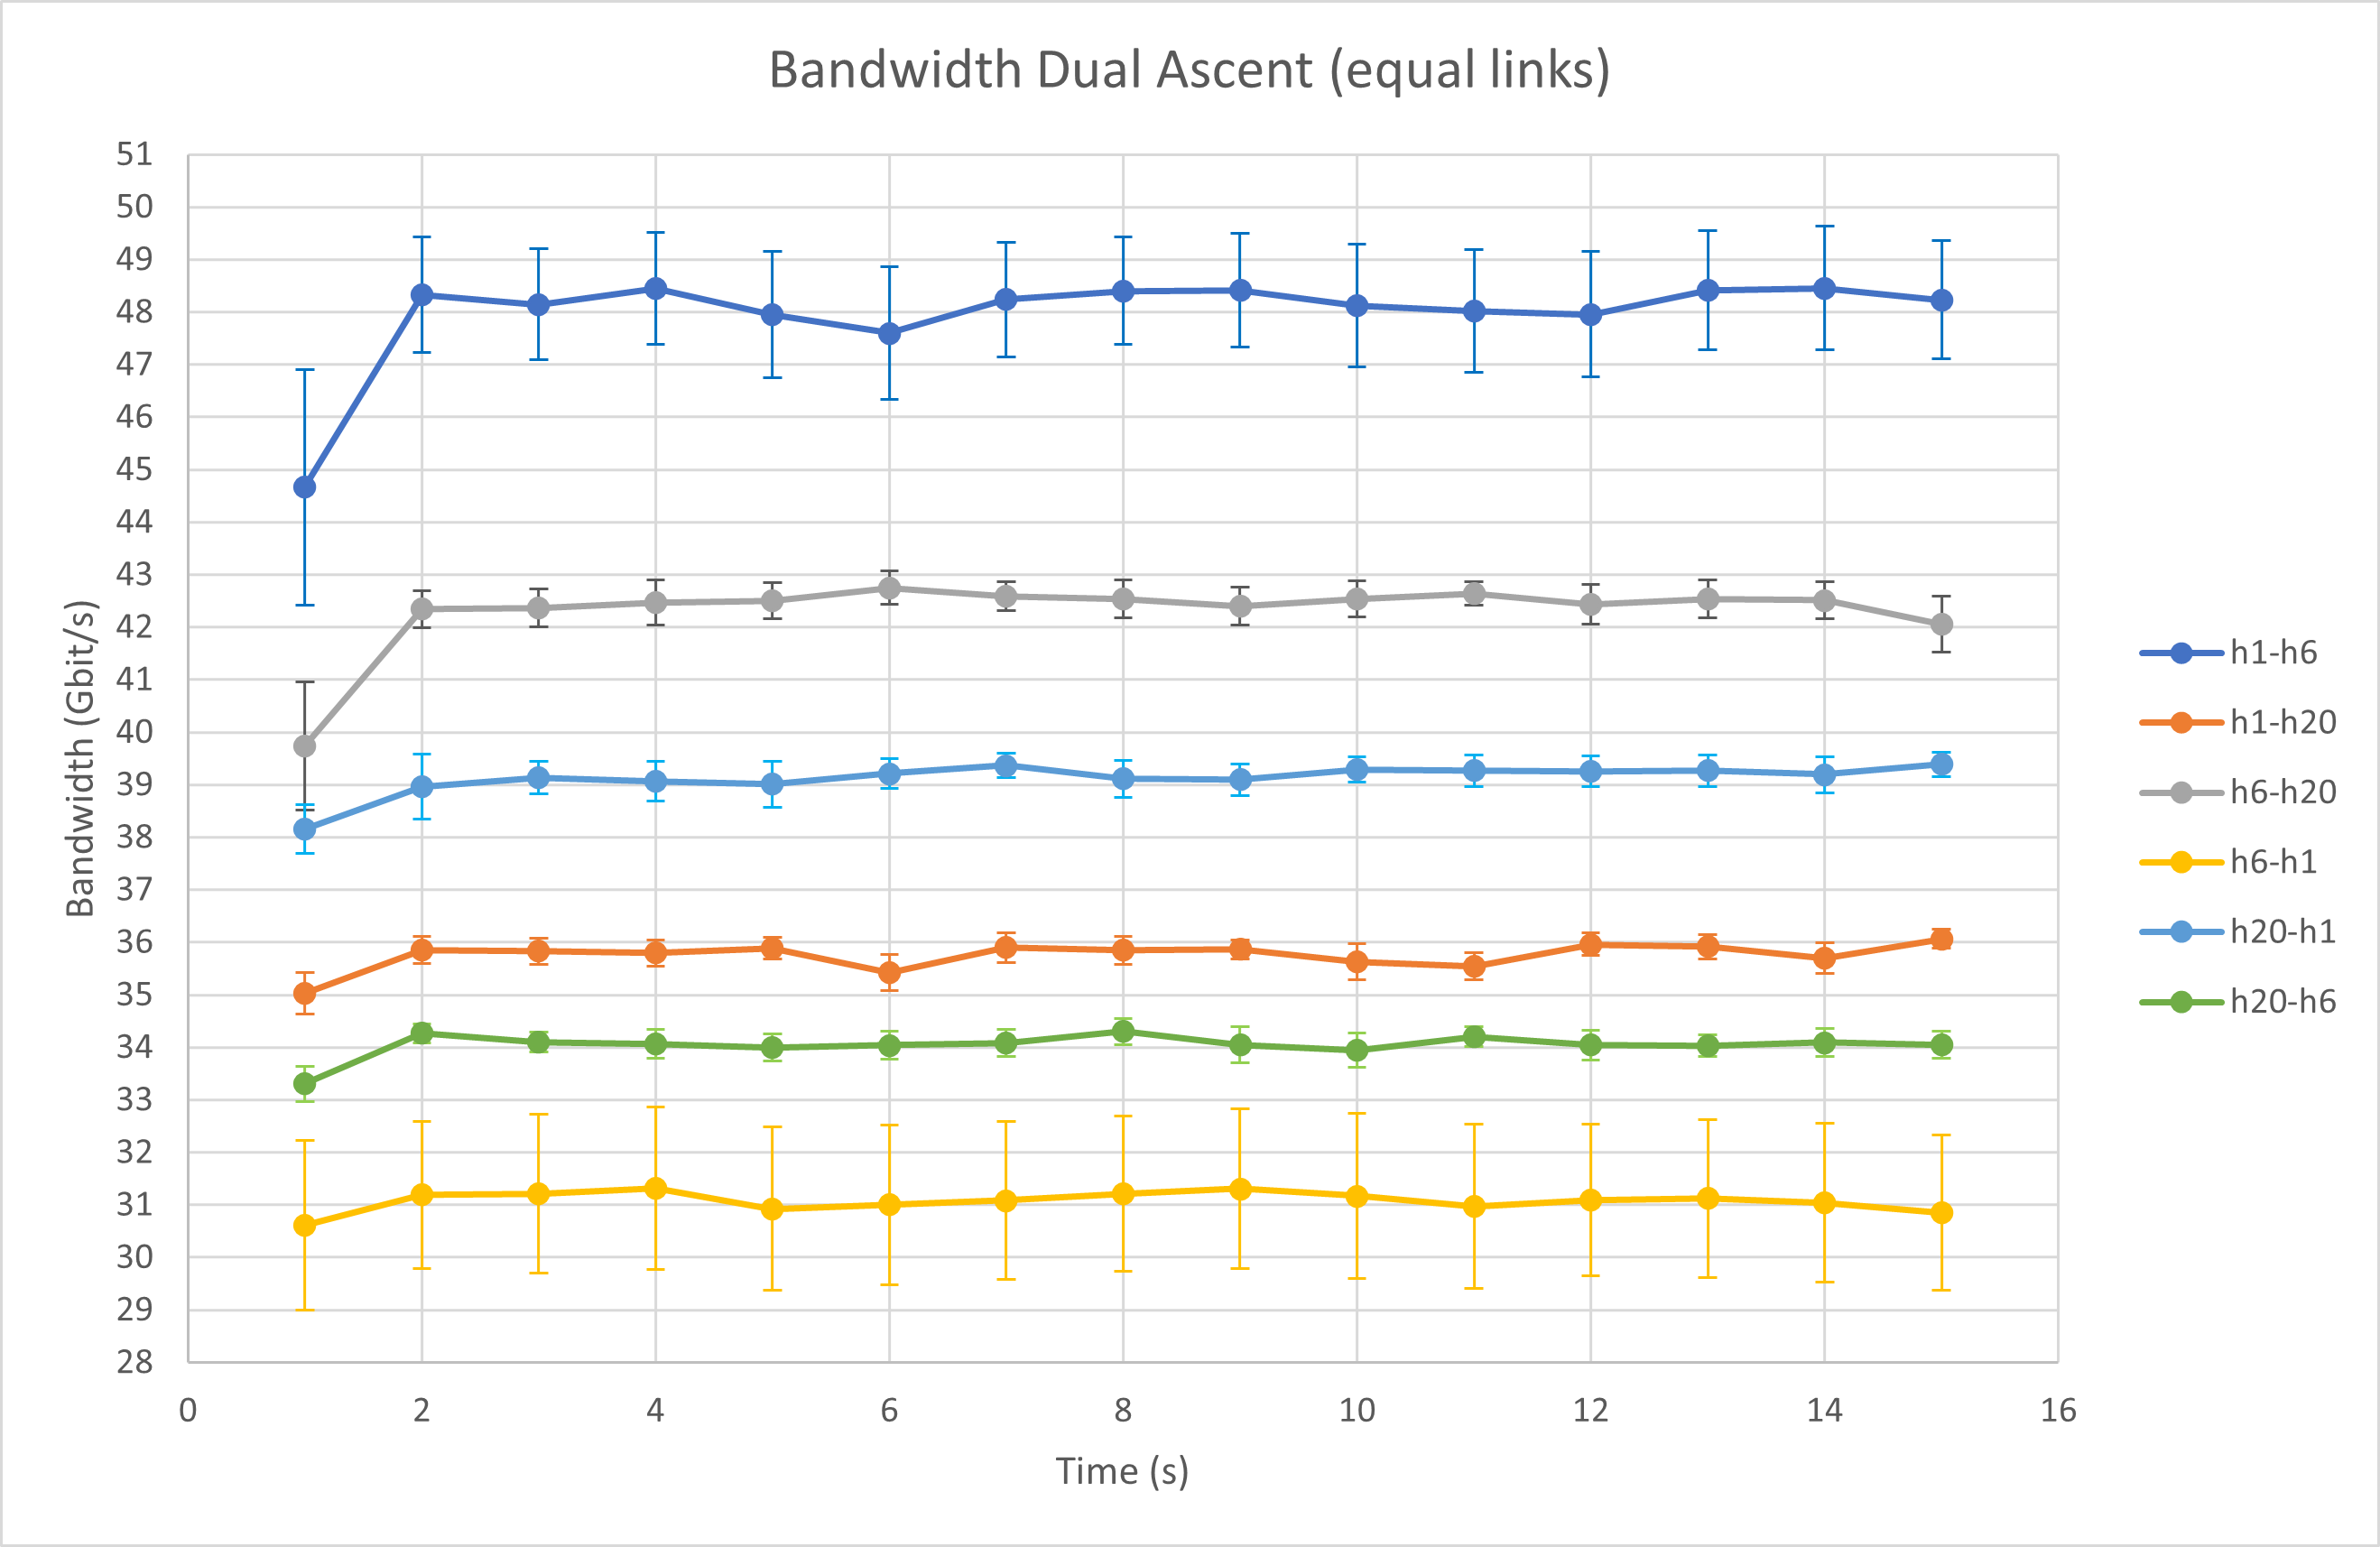
\includegraphics[width=\textwidth]{img/band-eq-dual.png}
		\caption{Throughput in time for Dual Ascent algorithm with equal
		link bandwidth}\label{subfig:band-eq-dual}
	\end{subfigure}
	\caption{Comparison of the host-to-host throughput when using Dijkstra
	and dual ascent}\label{fig:bandwidth-equallinks}
\end{figure}

To have a final result we have aggregated all the path's throughputs to show
what algorithm seems to be the best. As we can see from
\figref{fig:band-aggregate-eq}, Dijkstra has an average throughput in time
always better with respect to Dual Ascent (\(\SI{44}{\gigabits\per\second}\) vs
\(\SI{38.5}{\gigabits\per\second}\)), but both has a similar shape and setup time
(the throughput is lower in the first two seconds, due to TCP slow start).

\begin{figure}[hbt]
	\centering
	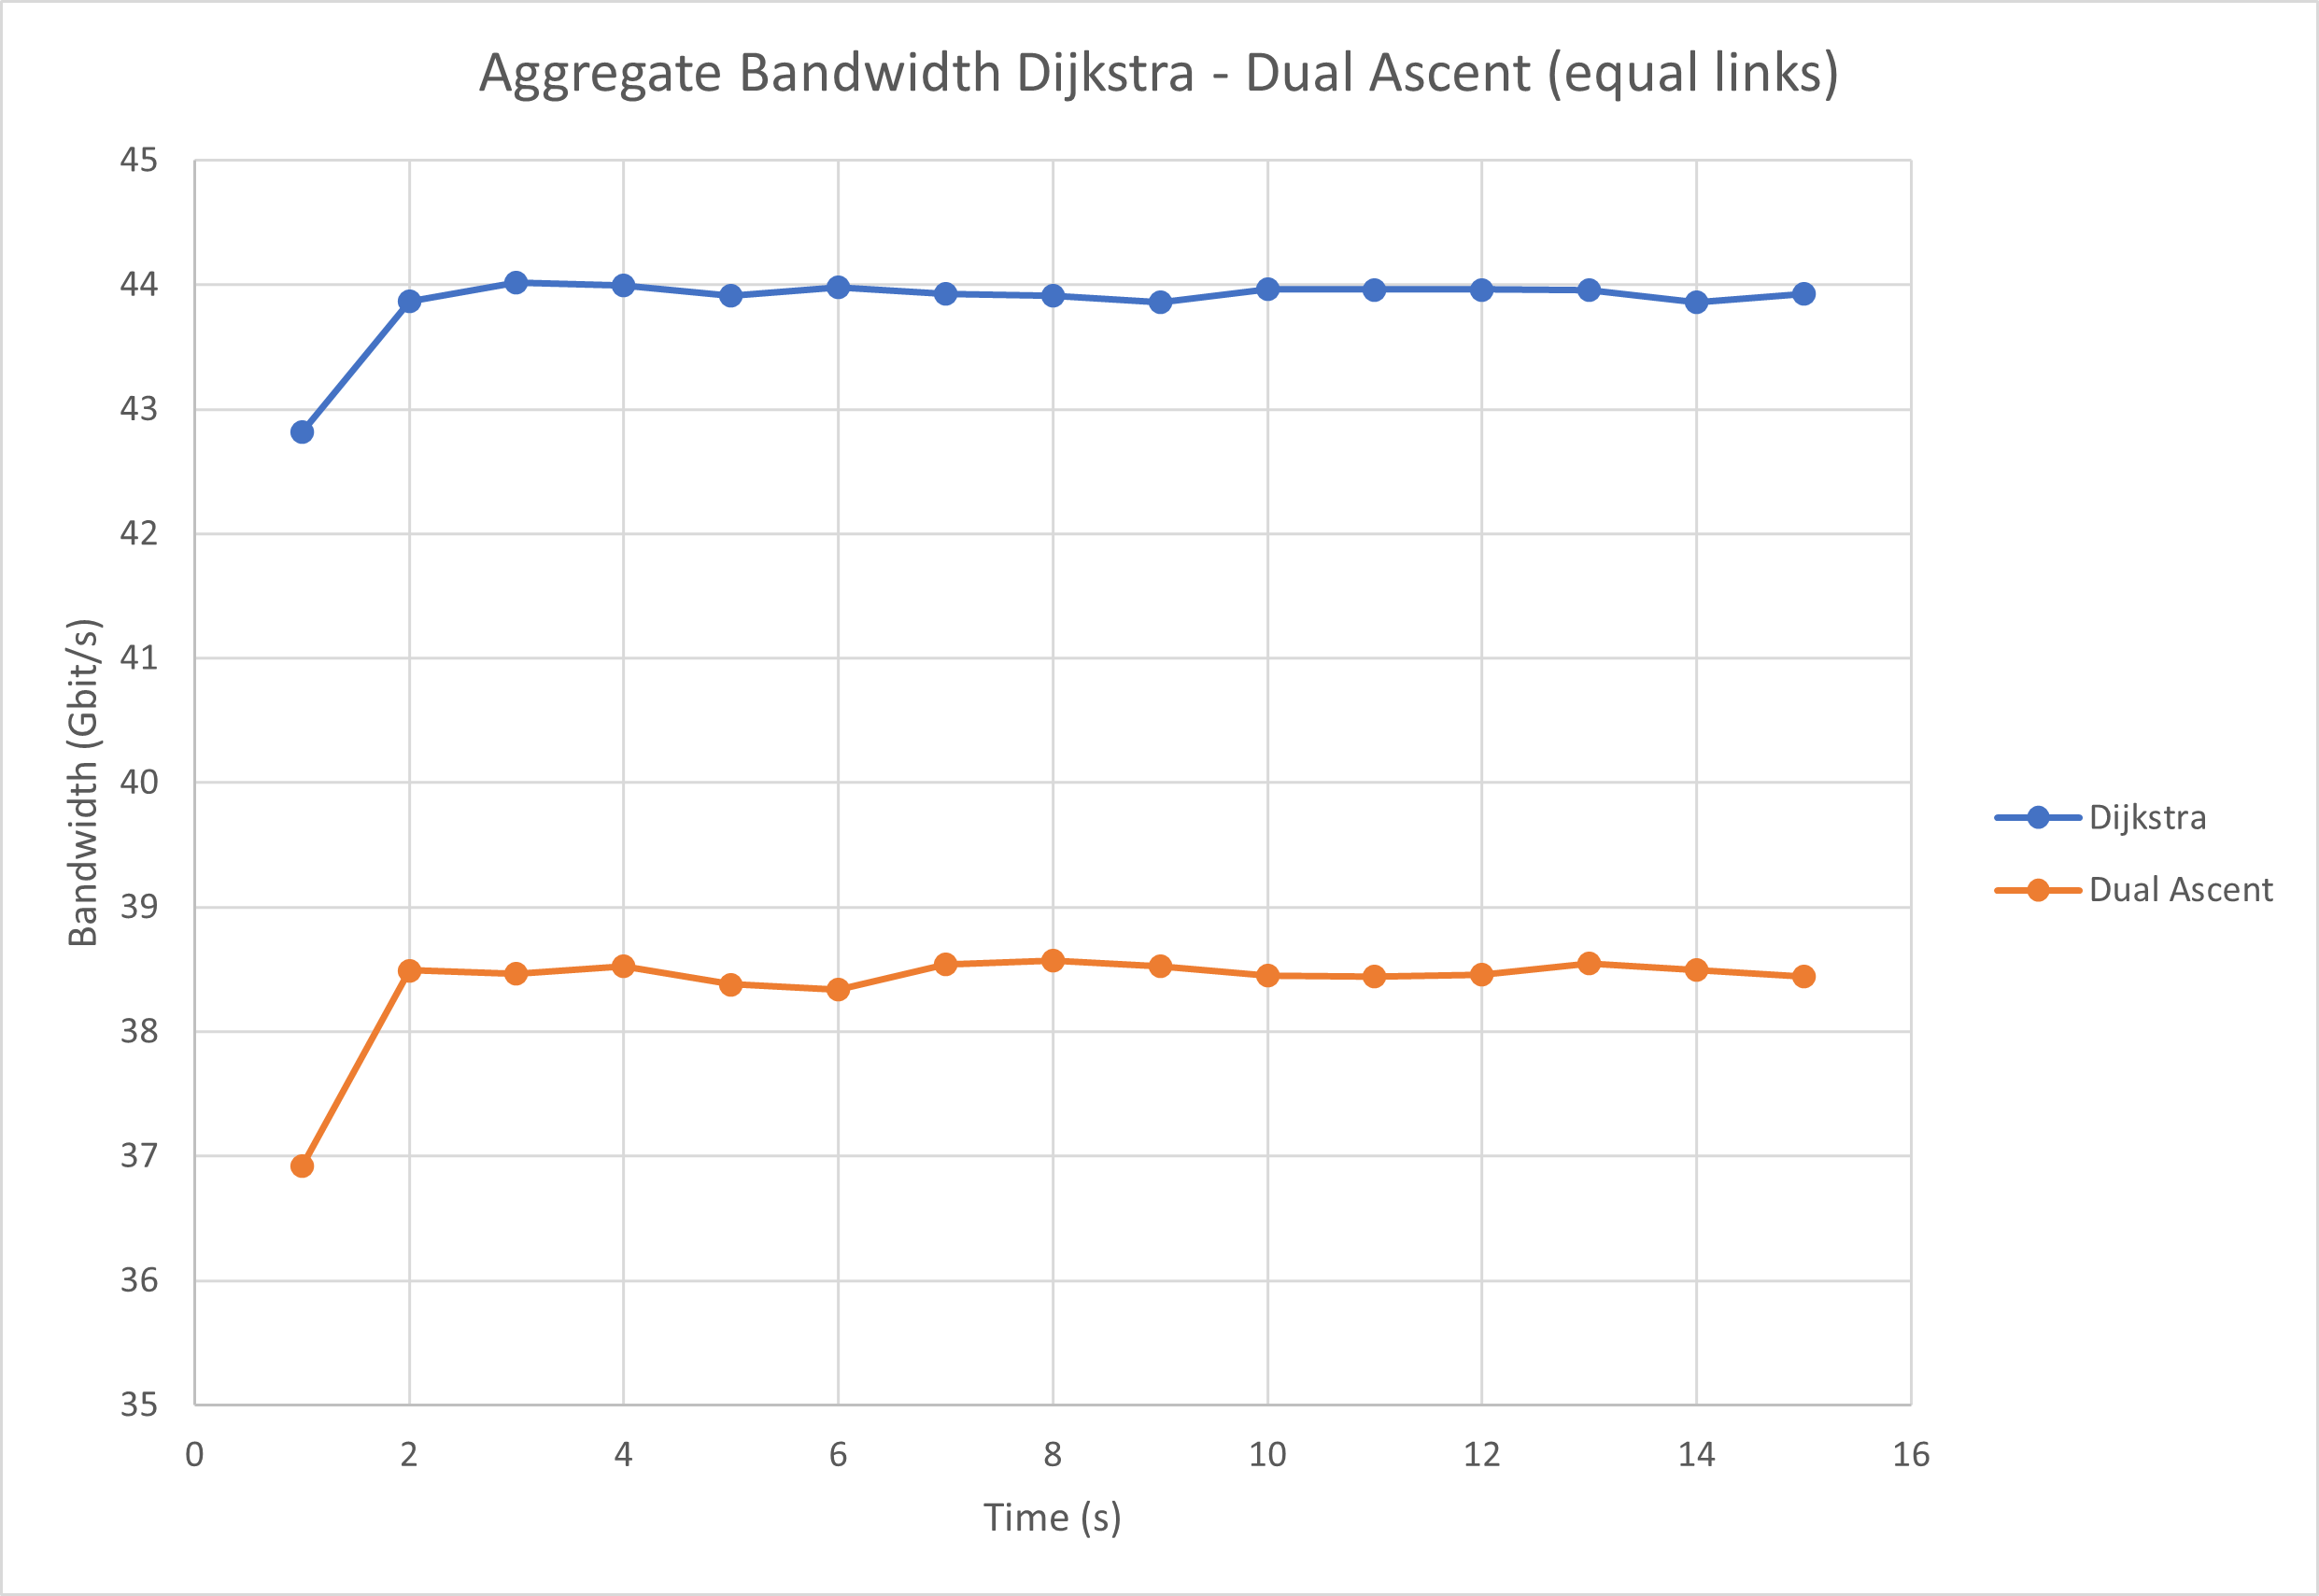
\includegraphics[width=\textwidth]{img/aggregate-band-eq.png}
	\caption{Aggregate mean for the throughput with equal starting
	bandwidth}\label{fig:band-aggregate-eq}
\end{figure}

\subsection{Different link bandwidth}

For this experiment links has different bandwidth, calculated using, for each
link, the sum of indexes of the attached switches (two for each link),
multiplied by a factor of 25 (in Mbits/s). In \figref{subfig:band-div-dijkstra}
we have the average throughputs in Dijkstra algorithm and in
\figref{subfig:band-div-dual} there is the analogue for the Dual ascent
algorithm.

\begin{figure}
	\centering
	\begin{subfigure}[b]{\textwidth}
		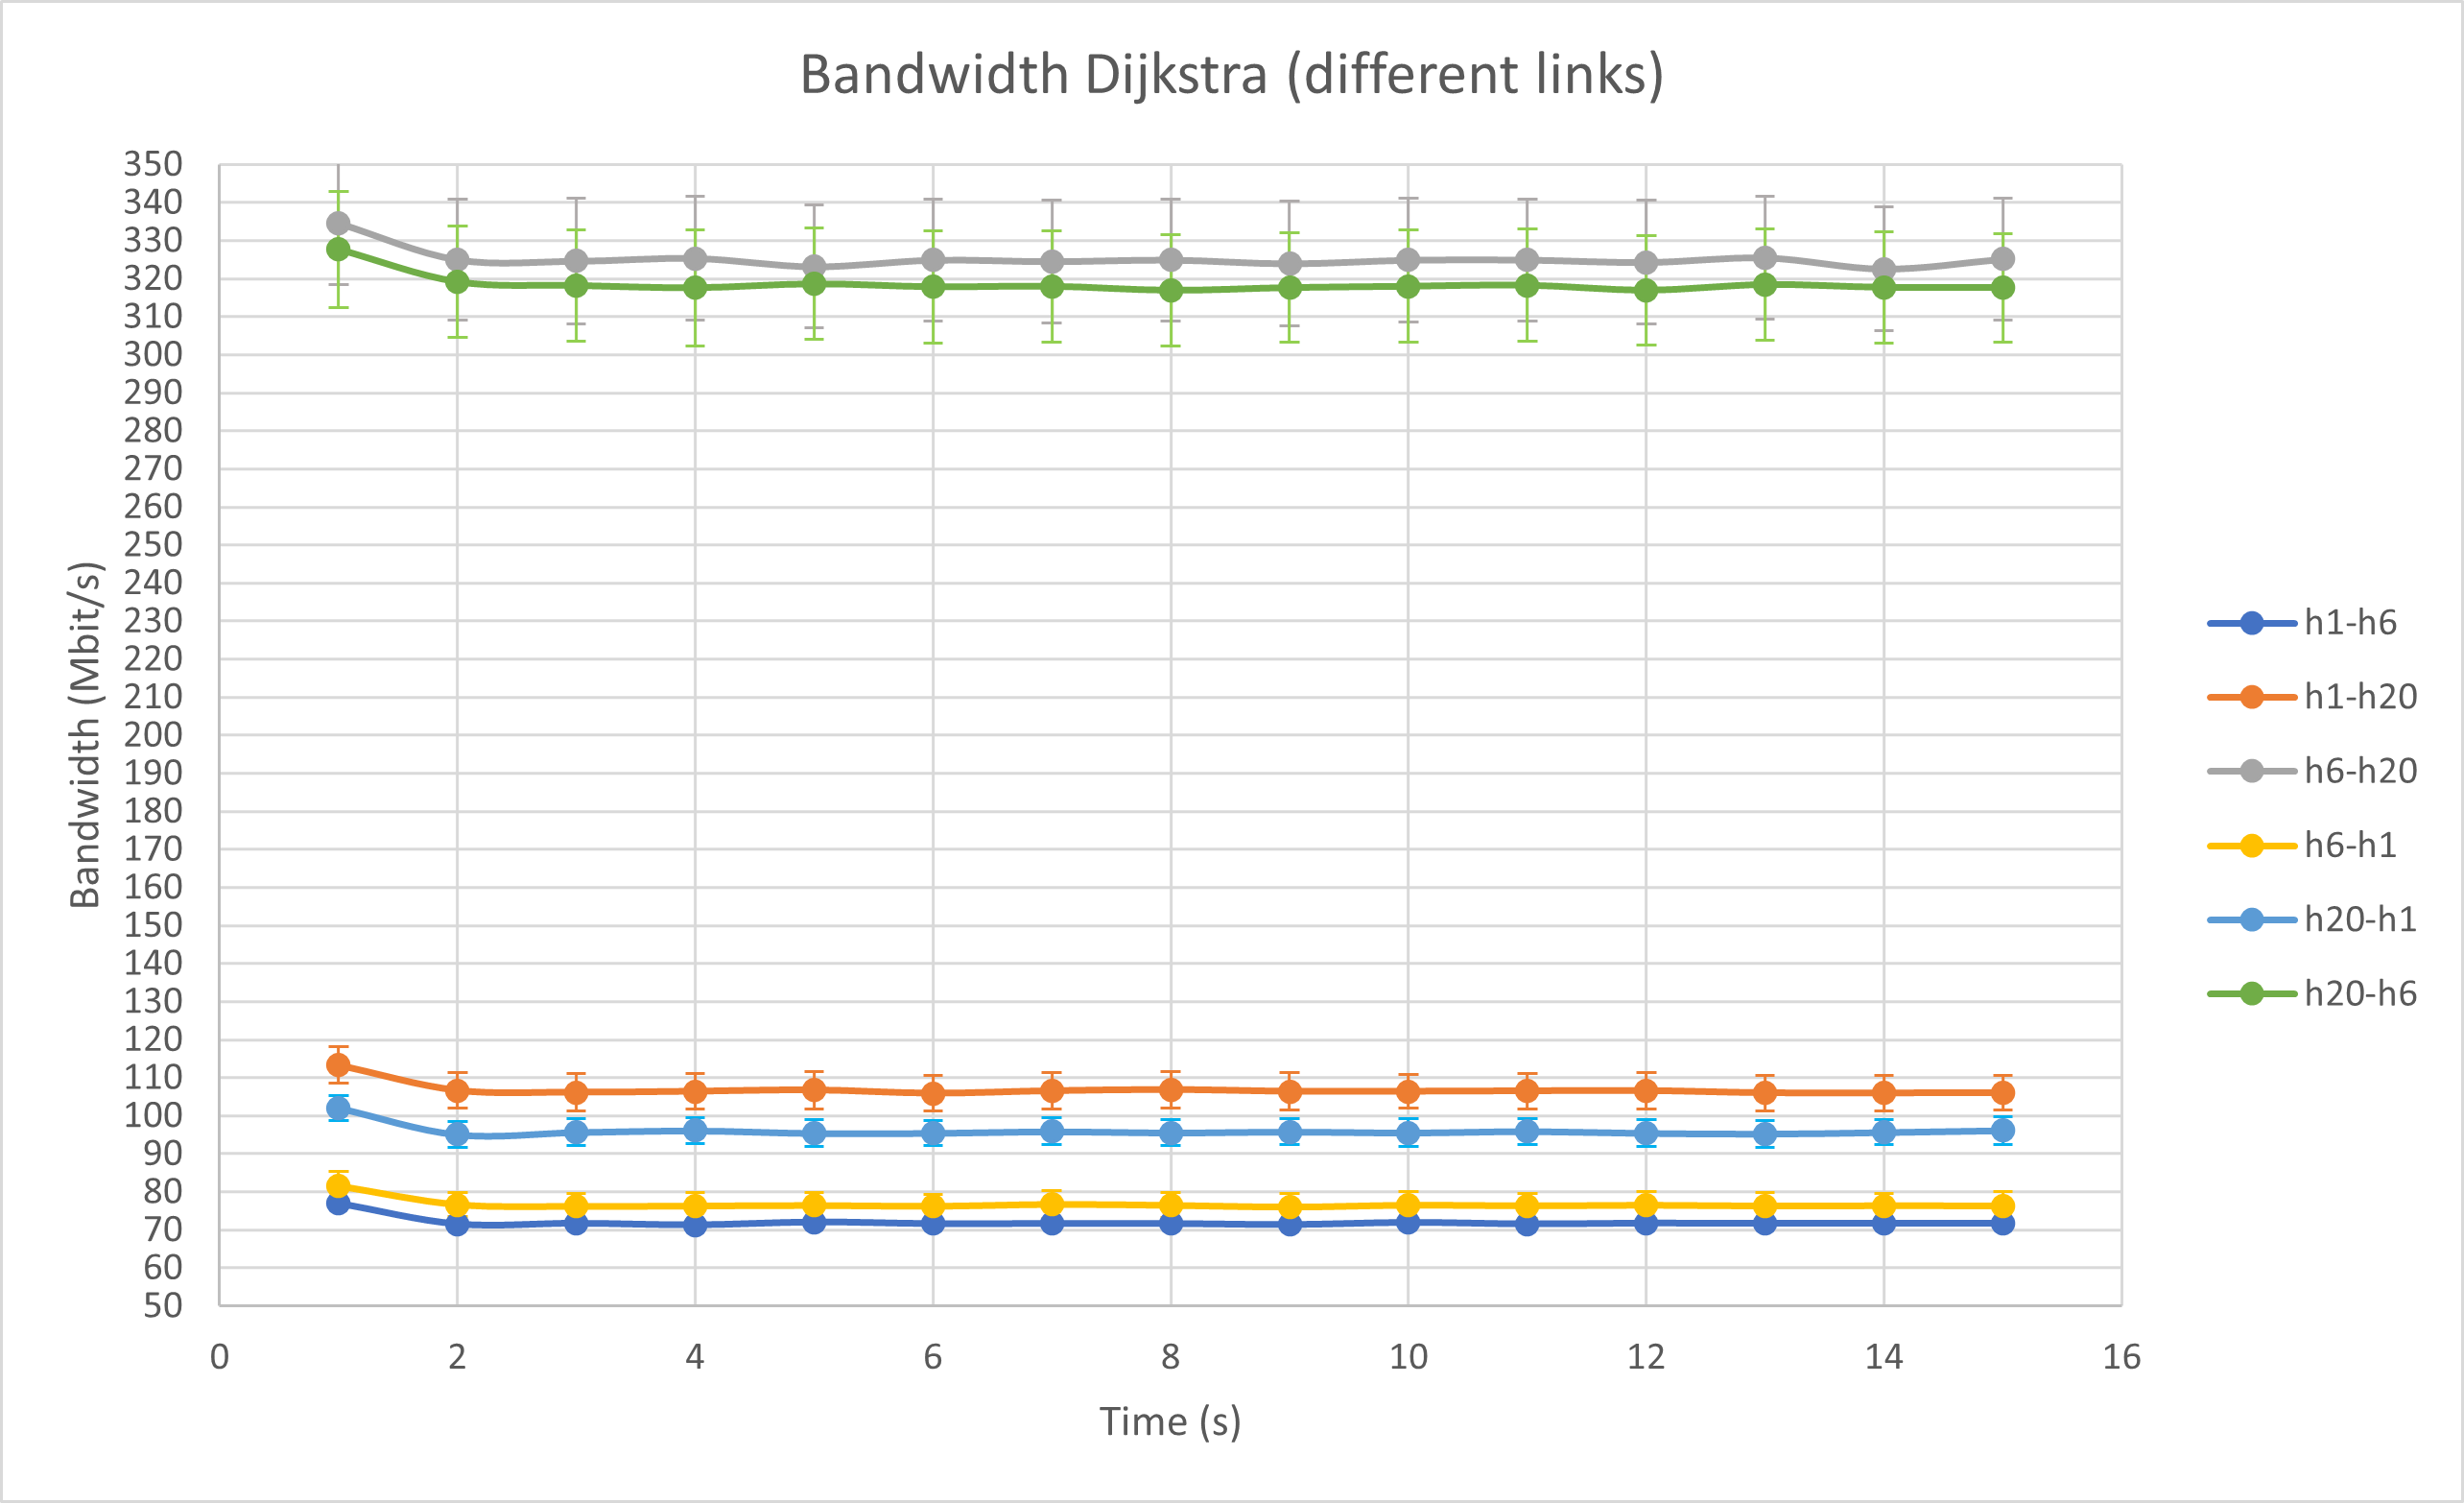
\includegraphics[width=\textwidth]{img/band-div-dijkstra.png}
		\caption{Throughput in time for Dijkstra algorithm with
		different link bandwidth}\label{subfig:band-div-dijkstra}
	\end{subfigure}
	\begin{subfigure}[b]{\textwidth}
		\centering
		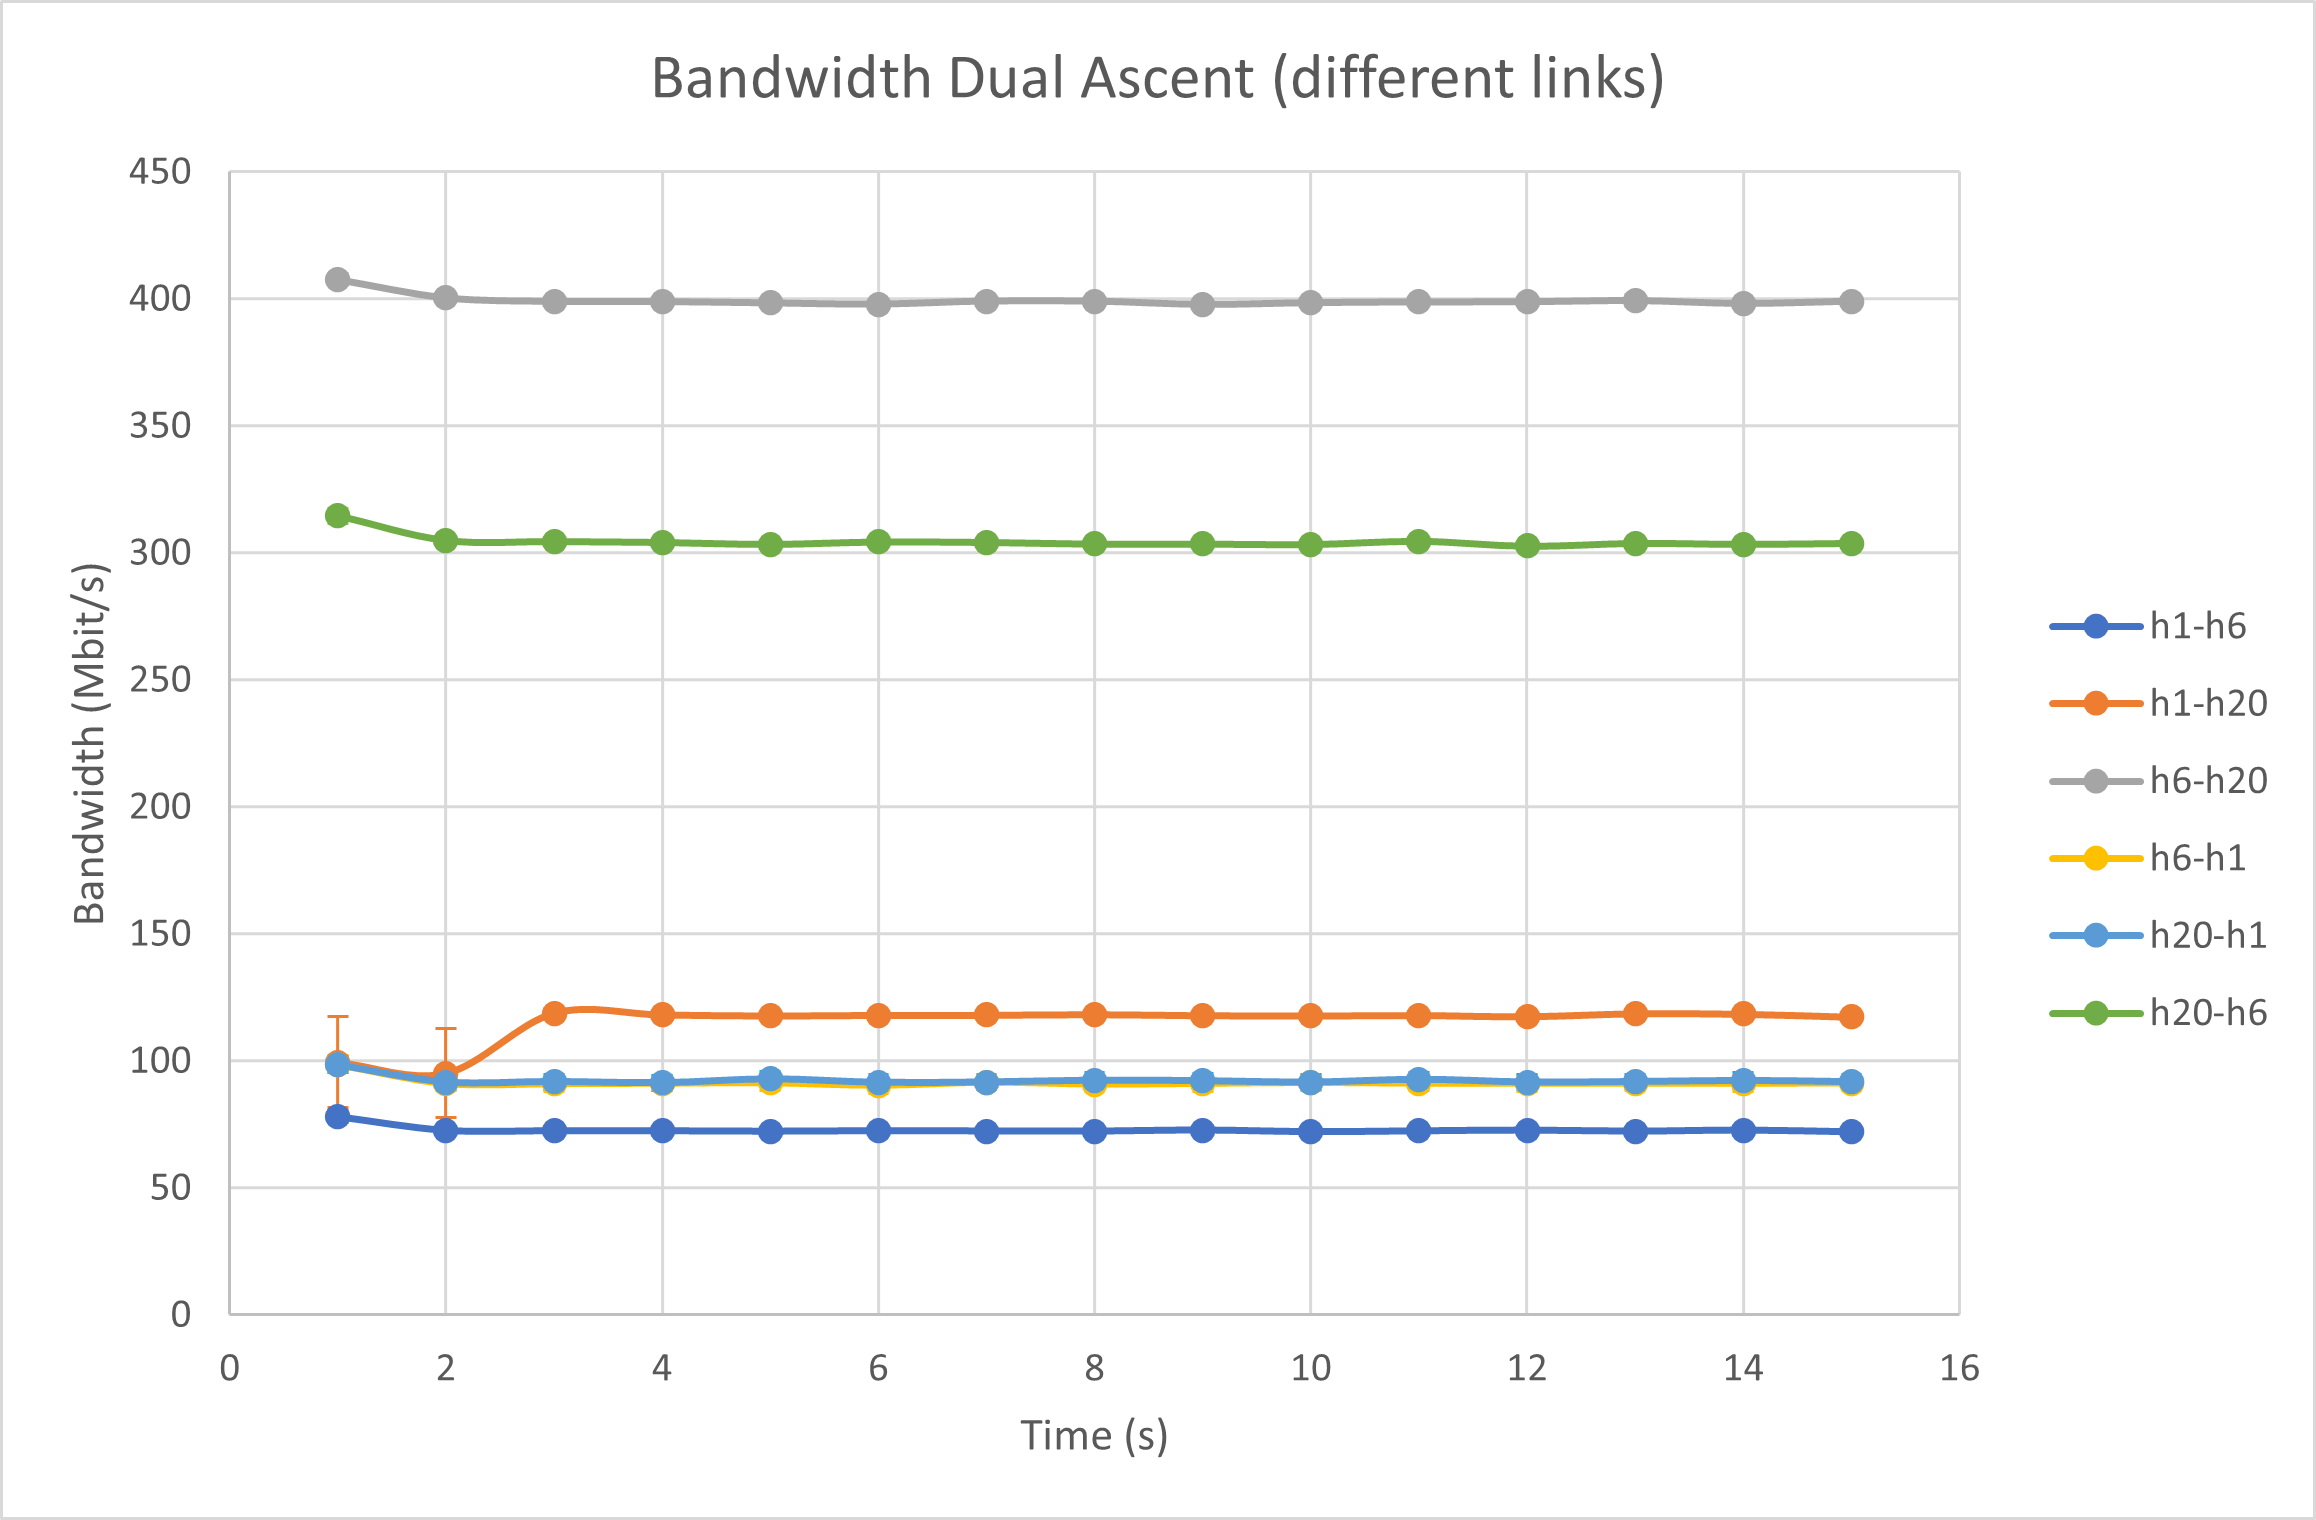
\includegraphics[width=\textwidth]{img/band-div-dual.png}
		\caption{Throughput in time for Dual Ascent algorithm with
		different link bandwidth}\label{subfig:band-div-dual}
	\end{subfigure}
	\caption{Comparison of the host-to-host throughput when using Dijkstra
	and dual ascent in the topology with links with different
	bandwidths}\label{fig:bandwidth-difflinks}
\end{figure}

The final aggregation, shown in \figref{fig:band-aggregate-div}, tells that in
this case Dual Ascent has an average throughput in time always better with
respect to Dijkstra (\(\SI{179}{\megabits\per\second}\) vs
\(\SI{165}{\megabits\per\second}\)), with a different shape only in the first
two seconds.

\begin{figure}
	\centering
	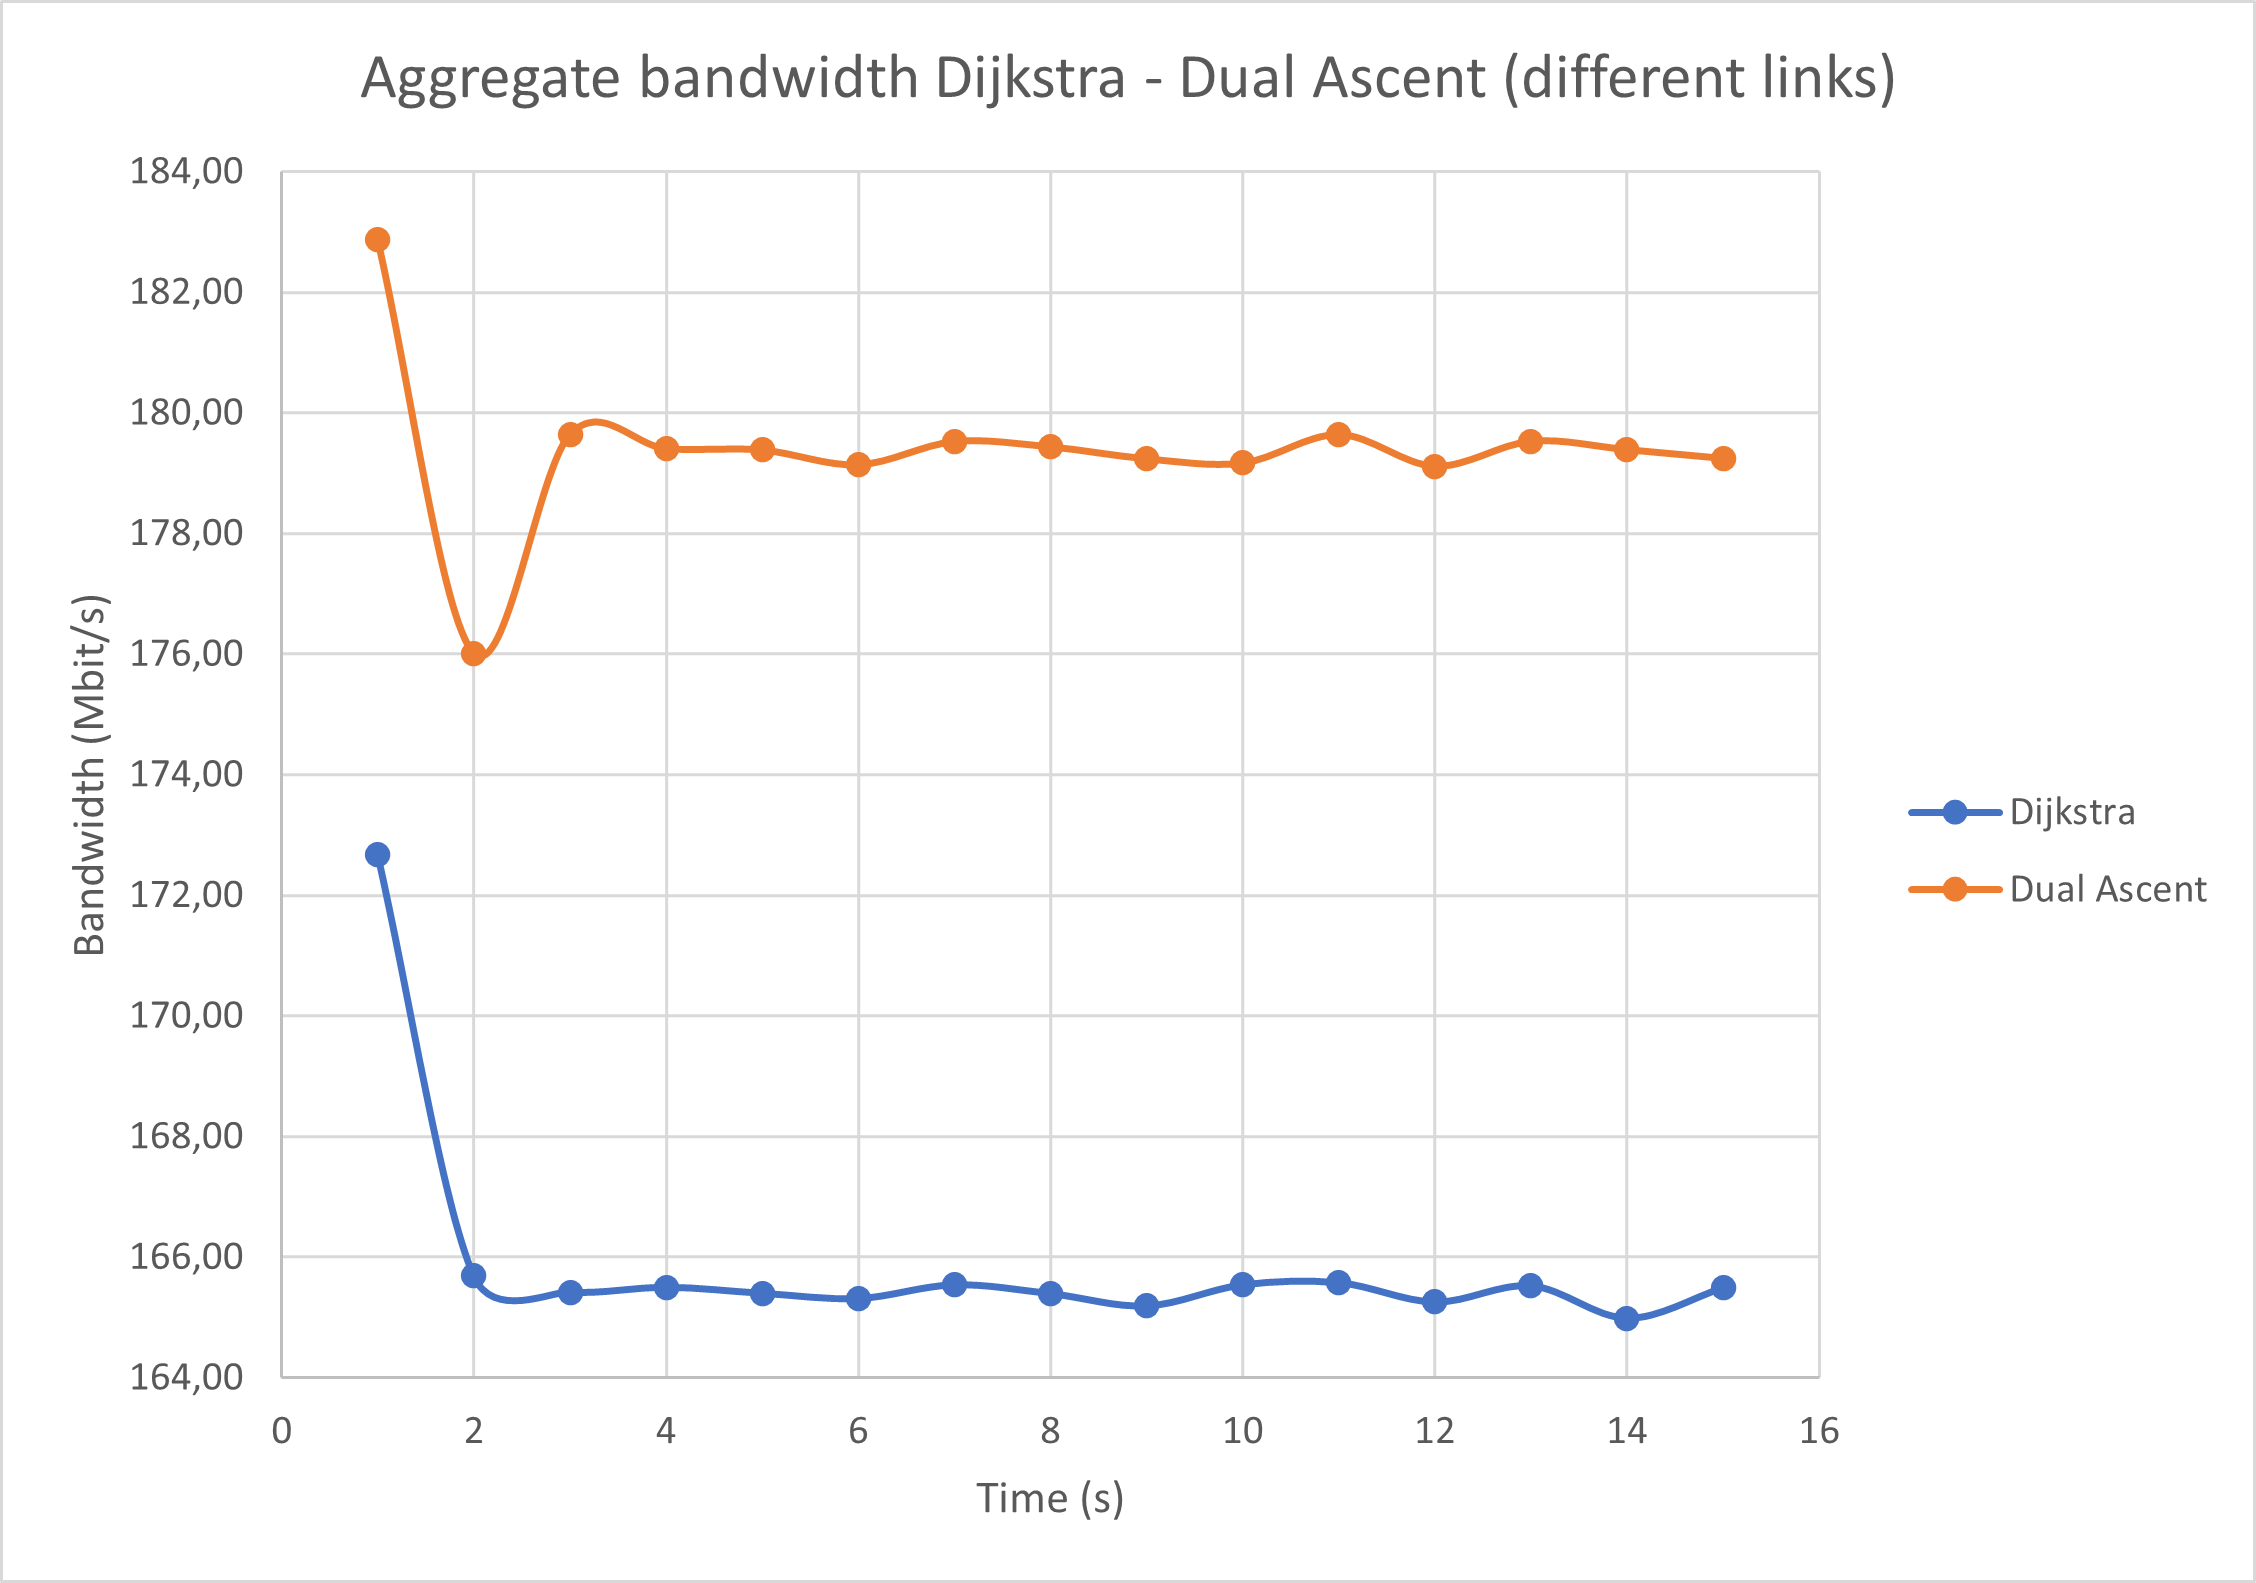
\includegraphics[width=\textwidth]{img/aggregate-band-div.png}
	\caption{Aggregate mean for the throughput with different
	bandwidth for links}\label{fig:band-aggregate-div}
\end{figure}

As we can see results are similar, because all the nodes are considered as
target nodes. So there isn't so many difference between the two algorithm and
this is shown by the fact that in one case Dijkstra is better and in the other
case it is not. We expect that changing topologies and link costs we get an
alternation of the better algorithm, based on the single situation. To have
generally different results we have to set some nodes as non-target, but this is
not supported by Floodlight as it wants to compute every time the broadcast tree
with all nodes in the network.
